
\vspace*{1mm}
In 2018, two prototype Crab Cavities ($\CC$s) were installed in the SPS to be tested for the first time with proton beams. A series of dedicated machine developemnt studies was carried out in order to validate their working principle and answer various beam dynamic questions. One of the operational issues that needed to be addressed concerned the expected emittance growth due to noise in their RF system, which is the main subject this thesis. As mentioned in Chapt... a theoretical model had already been developed and validated by trackig simulations~\cite{PhysRevSTAB.18.101001}. As a part of the first experiemental campaign with $\CC$s in SPS a dedicated experiment was conducted to benchmark these models with experimental data and confirm the analytical predictions. The objective of this chapter is to provide an overview of the general machine setup for the $\CC$ experiements and introduce the instruments and methods used for measuring the beam parameters of interest for the emittance growth studies.


The chapter is stractured as follows: Section~\ref{sec:CC_SPS_setup} describes the installation of the $\CC$s in the SPS and the experimental machine configuration. According to the theroetical model we need to measure the crab cavity voltatge, the emttance and the bunch lenth.


The use of the Head-Tail (HT) monitor as the main diagnostic device for measurement of the crabbing is presented in Section~\ref{sec:HT_info}. Last, the analysis of the HT measurements for the callibration of the $\CC$ voltage and the reconstruction of the crabbing are discussed in Sections~\ref{sec:Vcc_calibration} and~\ref{sec:Crabbing_reconstruction} respectively. test

\section{Crab Cavities in the SPS}\label{sec:CC_SPS_setup}

For the SPS tests two prototype $\CC$s of the Double Quorter Wave (DQW) type were fabricated by CERN and were assembled into the same cryomodule which is shown in Fig.~\ref{fig:DQW_cryomodule}~\cite{Zanoni:2017}. The cryomodule was installed in the SPS-LSS6 zone, Fig.~\ref{fig:CC_SPS_LSS6}, and was placed on a mobile transfer table~\cite{Calaga:2649807}. The table moved with high precision and without breaking the vaccum the cryomodule in the beam line for the $\CC$ tests and out of it for the usual SPS operation. The main parameters for the $\CC$ experiments in SPS are shown in Table~\ref{tab:SPS_CC_main}


\begin{figure}[h]
   \centering         
   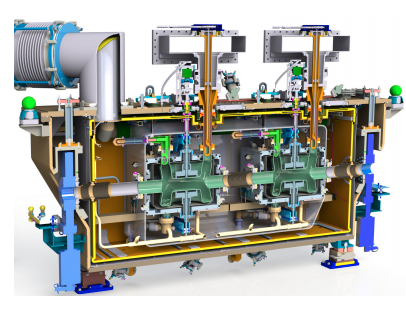
\includegraphics[width=0.8\textwidth]{images/Ch4/CC_cryomodule.png}
       \caption{Cut of the CC cryomodule~\cite{Zanoni:2017}.}
       \label{fig:DQW_cryomodule}
\end{figure}

\begin{figure}[h]
   \centering         
   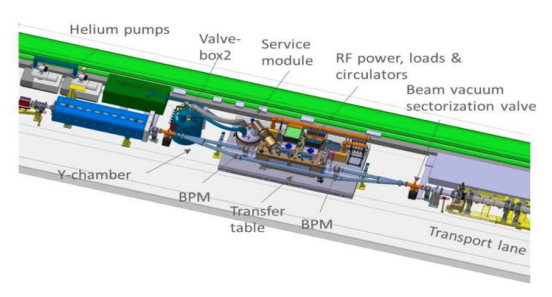
\includegraphics[width=0.8\textwidth]{images/Ch4/CC_location_SPS_LSS6.png}
       \caption{Installation of the cryomodule in the SPS-LSS6 zone~\cite{Calaga:2649807}.}
       \label{fig:CC_SPS_LSS6}
\end{figure}

\begin{table}[!hbt]
	\centering
   \caption{Parametes for the SPS CC tests}
	\begin{tabu} to \textwidth { X[c,m] X[c,m] X[c,m] X[c,m] X[c,m] X[c,m] }
		&&&&& \\[-6mm]
		\toprule \toprule
		\multicolumn{2}{l}{\textbf{Parameters}} &
		\multicolumn{2}{c}{\textbf{Units}} &
		\multicolumn{2}{c}{\textbf{Values}} \\
		\bottomrule
      \multicolumn{2}{l}{$\symE$} & \multicolumn{2}{c}{[GeV]} & \multicolumn{2}{c}{26, 270} \\
      \multicolumn{2}{l}{Main RF frequency} & \multicolumn{2}{c}{[MHz]} & \multicolumn{2}{c}{200} \\
      \multicolumn{2}{l}{$\Qx$ / $\Qy$} & \multicolumn{2}{c}{[-]} & \multicolumn{2}{c}{26.13 / 26.18 } \\
      %\arrayrulecolor{black!30}\midrule
      \midrule
      \multicolumn{2}{l}{} & 	\multicolumn{2}{c}{} & \multicolumn{1}{c}{\textbf{CC1}} & \multicolumn{1}{c}{\textbf{CC2}} \\
      \midrule
      \multicolumn{2}{l}{crabbing plane} & \multicolumn{2}{c}{[-]} & \multicolumn{1}{c}{vertical} & \multicolumn{1}{c}{vertical} \\
      
      \multicolumn{2}{l}{s-location} & \multicolumn{2}{c}{[m]} & \multicolumn{1}{c}{6312.72} & \multicolumn{1}{c}{6313.32} \\

      \multicolumn{2}{l}{$\VCC$, \footnotesize{MAX}} & \multicolumn{2}{c}{[MV]} & \multicolumn{1}{c}{4.3} & \multicolumn{1}{c}{4.3} \\

      \multicolumn{2}{l}{$\fCC$} & \multicolumn{2}{c}{[MHz]} & \multicolumn{1}{c}{400} & \multicolumn{1}{c}{400} \\

      \multicolumn{2}{l}{$\beta_{x, CC}$ / $\beta_{y, CC}$} & \multicolumn{2}{c}{[m]} & \multicolumn{1}{c}{29.24 / 76.07} & \multicolumn{1}{c}{30.31 / 73.82} \\

      \multicolumn{2}{l}{$\alpha_{x, CC}$ / $\alpha_{y, CC}$} & \multicolumn{2}{c}{[m]} & \multicolumn{1}{c}{-0.88 / 1.9} & \multicolumn{1}{c}{-0.91 / 1.86} \\

      \multicolumn{2}{l}{$D_{x, CC}$ / $D_{y, CC}$} & \multicolumn{2}{c}{[m]} & \multicolumn{1}{c}{-0.48 / 0} & \multicolumn{1}{c}{-0.5 / 0} \\
      \arrayrulecolor{black}\bottomrule
 
	\end{tabu}
   \label{tab:SPS_CC_main}
\end{table}


%\large{\textbf{Operational considerations}}\\
\subsection{Operational considerations}

For the beam tests with the $\CC$s in the SPS the approach regarding the energy ramp and the adjustment of the phasing with the main RF system needed to be evaluated and they are briefly discussed here.


\normalsize{\textbf{Energy ramp}}\\
SPS recieves the beam at 26\,GeV. It was observed that if the ramp to higher energies was performed with the $\CC$ on, the beam was lost while crossing one of the vertical betatron sidebands due to resonant excitation~\cite{Rama_Paris_persentation}. Therefore, it was established that the acceleration has to be performed with the $\CC$ off and its voltage must be set up only after the energy of interest has been achieved. It should be noted here that this will be the approach also for the HL-LHC.

\normalsize{\textbf{Crab Cavity - main RF synchronisation}}\\
Another issue of concern was the fact that the $\CC$ operate at the fixed frequency of 400\,MHz while the SPS main RF system operates at 200\,MHz.
In order to make sure that the beam will experience the same effect from the $\CC$ each turn the SPS main RF has to be re-phased such as it becomes synchronous with the crabbing signal. For studies at the injection energy of 26\,GeV this synchronisation took place shortly after the injection. For studies at 270\,GeV, like the emittance growth measurements, the synchronisation took place at the end of the ramp shortly after the cavity was switched on~\cite{BE_seminar}.


\section{The Head-Tail monitor}\label{sec:HT_info}
The HT monitor was the main diagnostic device deployed for the callibration of the $\CC$ voltage. Additionally, it was used for the measurement and the physical illustration of the crabbing. This made it a very useful tool in the time of the experiments as it provided a direct evaluation of the effect of the $\CC$ kick on the beam. The HT monitor was originally designed for measuring chromaticity and transverse isntabilities. Therefore its use as a crabbing diagnostic is explained here. The methods and procedures described in this section were developed at CERN and they are described here for the completness of the thesis.

 In the first part of this section some general information on the instrument along with example signals will be presented. Subsequently, the post processing of the HT signal in the presence of the $\CC$s and the method for the illustrating the crabbing will be discussed. Last, the callibration of the $\CC$ voltage is described. The experiemental data presented in this section were acquired at the SPS injection energy of 26\,GeV with only one $\CC$, $\CC$1, at $\phiCC=0$ for simplicity. This energy option was chosen as the effect of $\CC$ kick on the beam is stronger and thus more visible than in higher energies.



\normalsize{\textbf{The Heat-Tail monitor}}\\
\begin{figure}[h]
   \centering         
   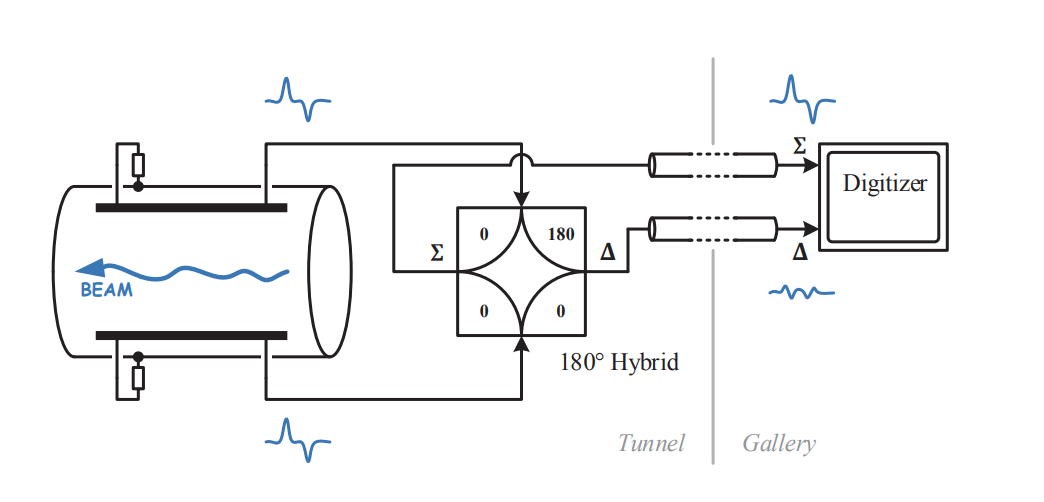
\includegraphics[width=0.8\textwidth]{images/Ch4/SPS_HT_monitor_diagram_modified.png}
       \caption{Diagram of the SPS HT monitor~\cite{Levens:2313358}.}
       \label{fig:SPS_HT_diagram}
\end{figure}
A standard beam position monitor (BPM) measures the bunch centroid position in the transverse planes at every passage of the beam. The HT monitor is a high bandwidth version of a standard BPM and can measure the transverse offset within the bunch, which makes it ideal for the measurement of the crabbing. Its reading consists of the sum $\Sigma$ and the  difference $\Delta$ of the electrode signals of a straight stripline coupler (Fig.~\ref{fig:SPS_HT_diagram})~\cite{Jones:987561, Levens:2313358}. The $\Sigma$ signal is the longitudinal line density while the $\Delta$ signal corresponds to the intra-bunch offset. Example signlas obtained from the HT monitor are displayed in Fig.~\ref{fig:HT_example_acq_singleTurn}-~\ref{fig:HT_example_acq_multTurns_2D}.


\begin{figure}[!h]
   \centering         
   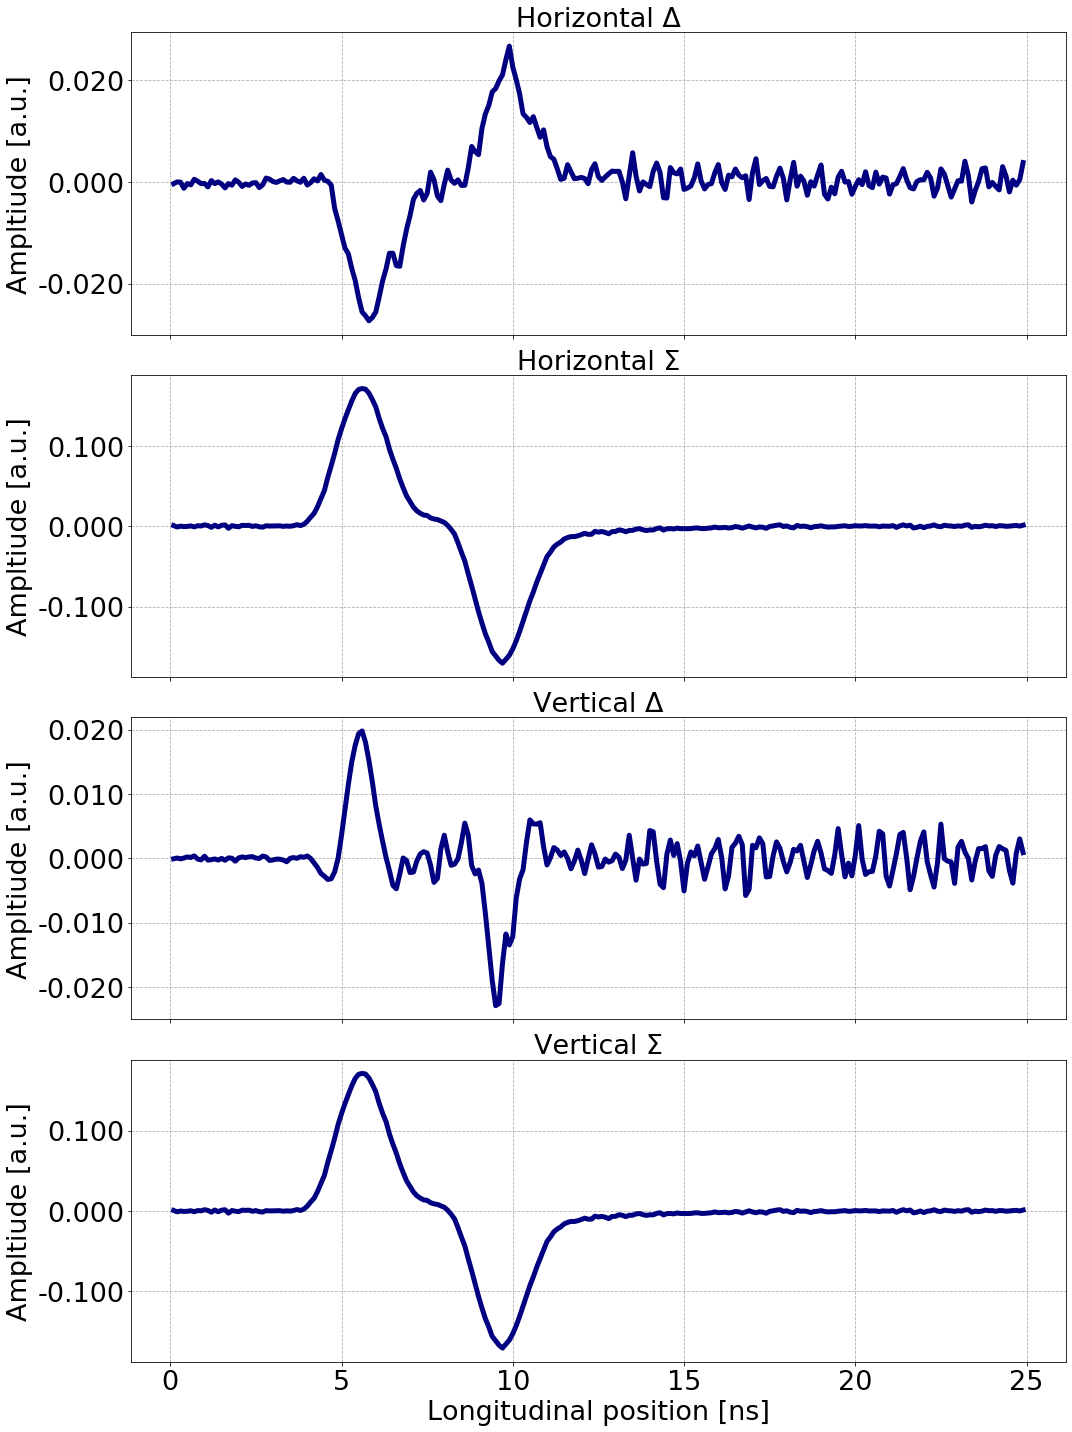
\includegraphics[width=0.8\textwidth]{images/Ch4/HT_1D__20180530_135105_exampleAcq_4thesis_turn3000.png}
       \caption{Raw example $\Delta$ and $\Sigma$ signals obtained from the HT monitor for a window of 25\,ns, acquired in a single SPS revolution.}
       \label{fig:HT_example_acq_singleTurn}
\end{figure}

\begin{figure}[!h]
   \centering         
   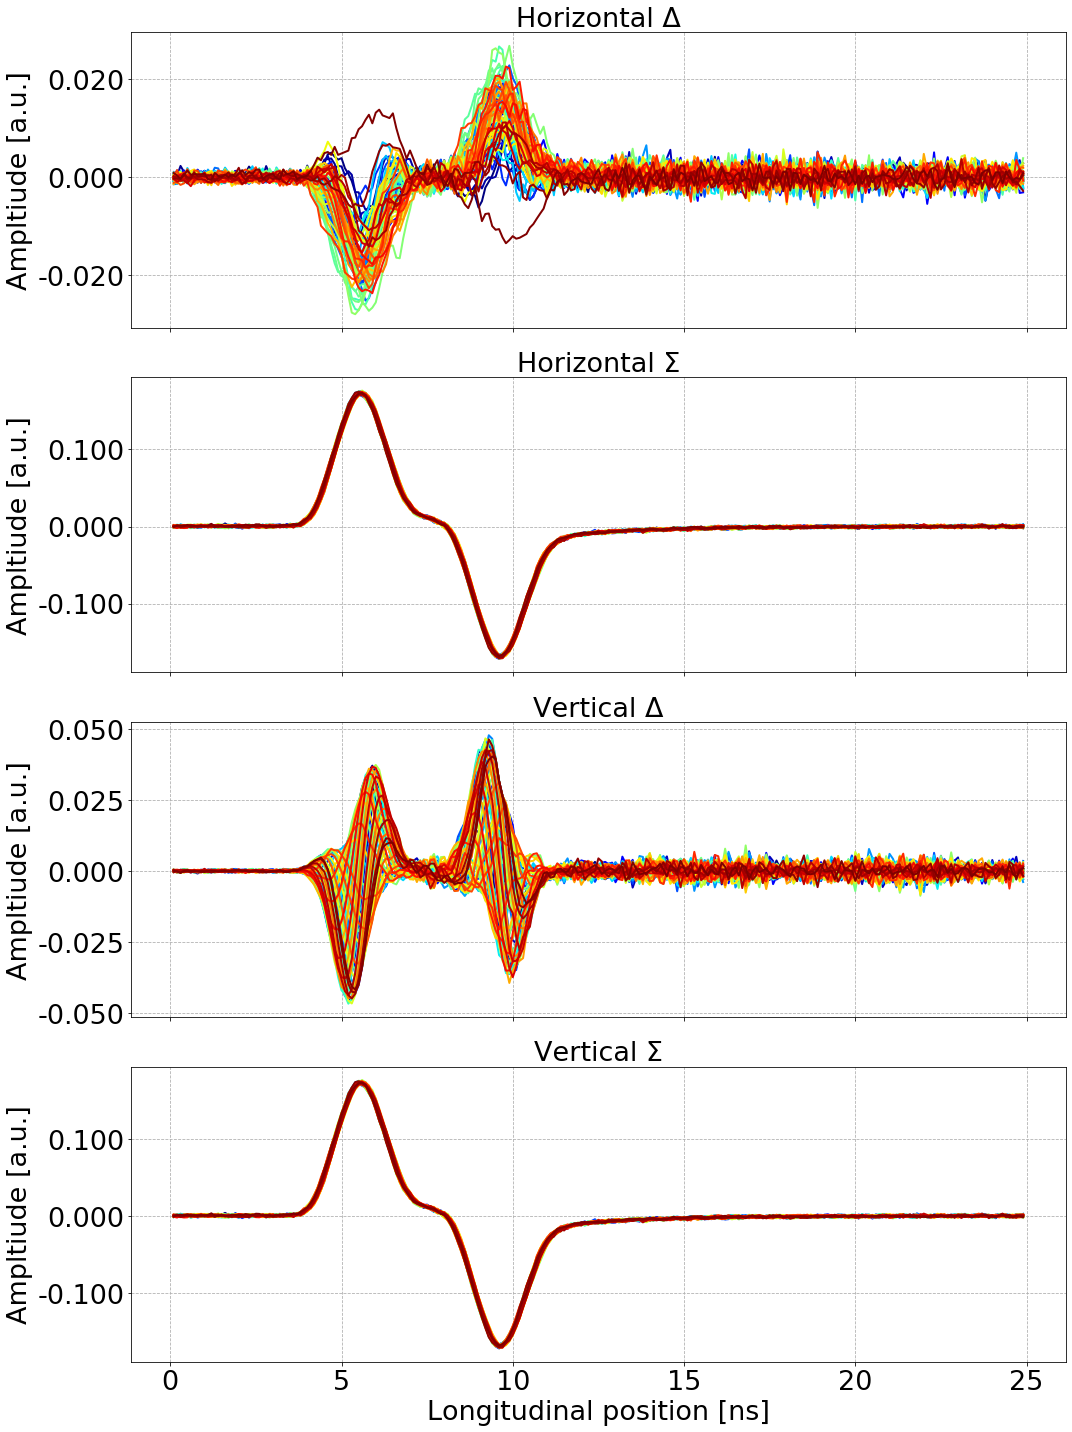
\includegraphics[width=0.8\textwidth]{images/Ch4/HT_1D__20180530_135105exampleAcq_4thesis_turnsStart0_Stop6000_step100.png}
       \caption{Example $\Delta$ and $\Sigma$ signals obtained from the HT monitor for a window of 25\,ns, acquired over several SPS revolutions. The color code indicates the different turns around the machine.}
       \label{fig:HT_example_acq_multTurns}
\end{figure}


\begin{figure}[!h]
   \centering         
   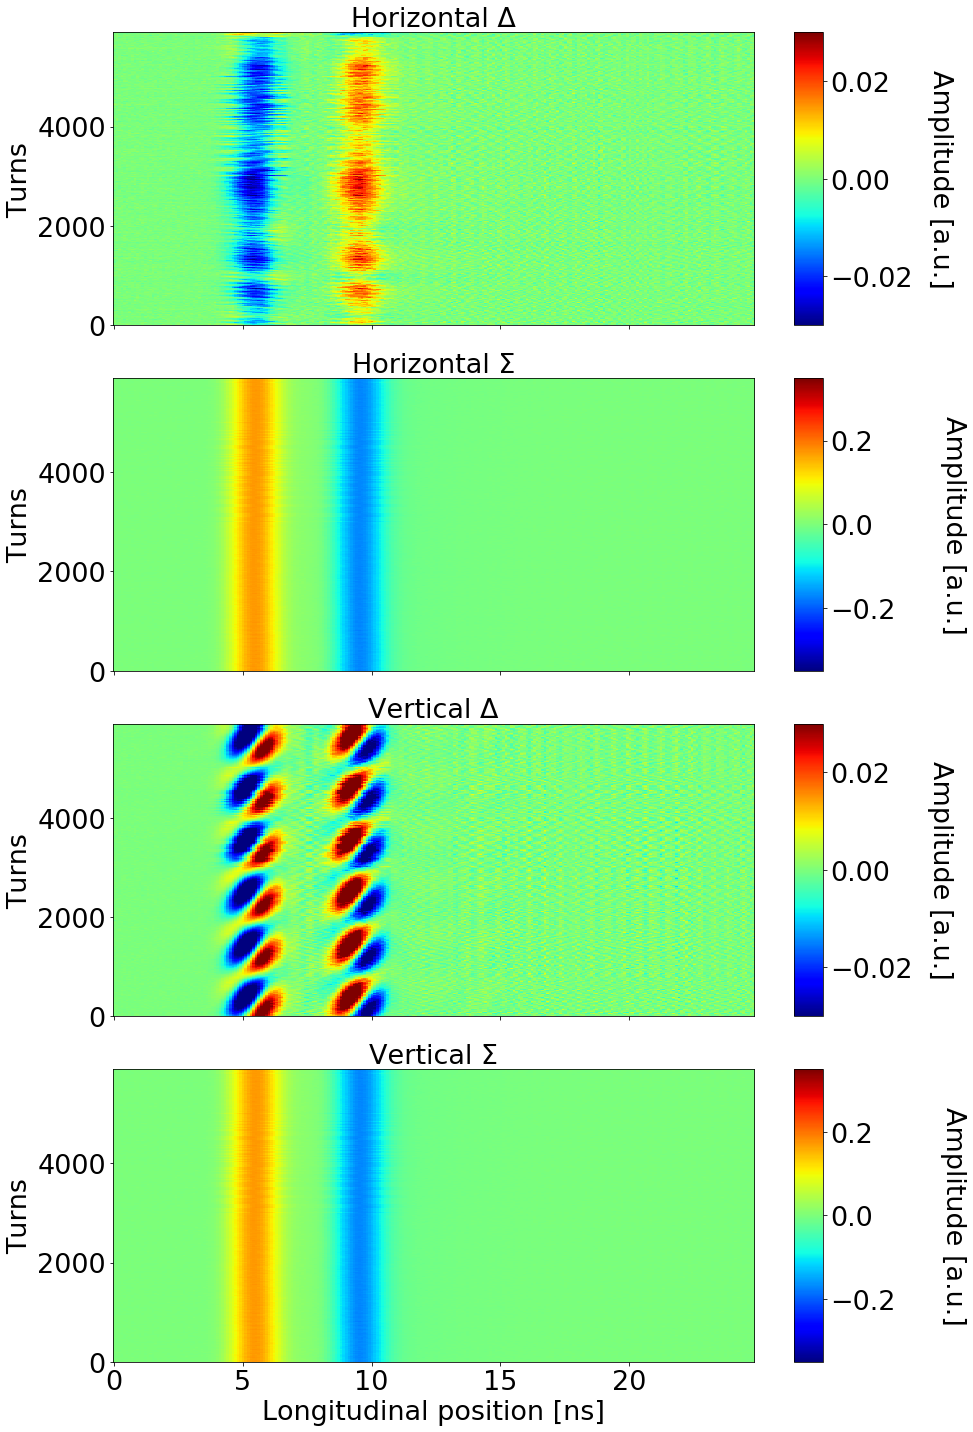
\includegraphics[width=0.8\textwidth]{images/Ch4/HT_2D__20180530_135105_colorbar.png}
       \caption{2D representation of example $\Delta$ and $\Sigma$ signals obtained from the HT monitor for a window of 25\,ns, acquired over several SPS revolutions.}
       \label{fig:HT_example_acq_multTurns_2D}
\end{figure}

In particular, Fig.~\ref{fig:HT_example_acq_singleTurn} and Fig.~\ref{fig:HT_example_acq_multTurns} illustrate the signal acquired over a single and multiple turns of the bunch around SPS respectively. The part of the signal after $\sim$ 9\,ns is just the reflected pulse of the bunch signal from the opposite end of the stripline. Moreover, Fig.~\ref{fig:HT_example_acq_multTurns_2D} shows a 2D representation of the HT monitor reading. It is worth mentioning already that in the specific example a clear periodic oscillation of the vertical intra-bunch offset (vertical $\Delta$) signal is observed. This is a result of the main RF system not being synchronous with the  $\CC$  frequency. 


\normalsize{\textbf{Heat-Tail monitor baseline correction}}\\
One issue of concern at that point was the correction of the $\Delta$ signal  baseline due to orbit offsets and non-linearities of the instrument~\cite{Levens:2313358}.  %present due to both the beam orbit offset in the head-tail pick-up and non-linearities of the hybrids, needs to be removed. https://accelconf.web.cern.ch/ibic2016/papers/thal02.pdf
Normally, the correction is achieved by computing the mean of the $\Delta$ signals over all turns and then subtracting this static offset from the signal of each turn. However, in the SPS tests, where the $\CC$s are well synchronised with the main RF system (Section~\ref{sec:CC_SPS_setup}), the crabbing signal is also a static intra-bunch position offset and thus would also be removed with the usual method.

Therefore, for the $\CC$ experiments a reference measurement had first to be made with the $\CC$ unsynchronised. The mean of the $\Delta$ signal over this reference period was the baseline which then was subtracted from the $\Delta$ signals acquired after the synchronisation (Fig~\ref{fig:HT_baseline_correction}). The datasets before and after synchronisation are easily distinguishable in the 2D HT monitor reading as displayed in Fig.~\ref{fig:HT_baseline_correction_measurements_2D}

\begin{figure}[!h]
   \centering         
   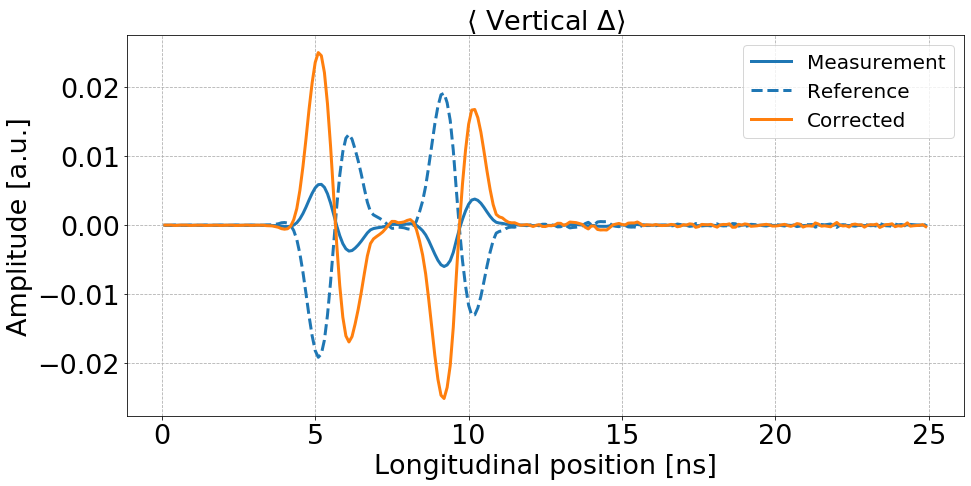
\includegraphics[width=0.8\textwidth]{images/Ch4/HT_measures_vs_reference_vs_corrected__20180530_135105_baseline_correction.png}
       \caption{HT monitor baseline correction for the SPS CC tests.}
       \label{fig:HT_baseline_correction}
\end{figure}

\begin{figure}[!h]
   \centering         
   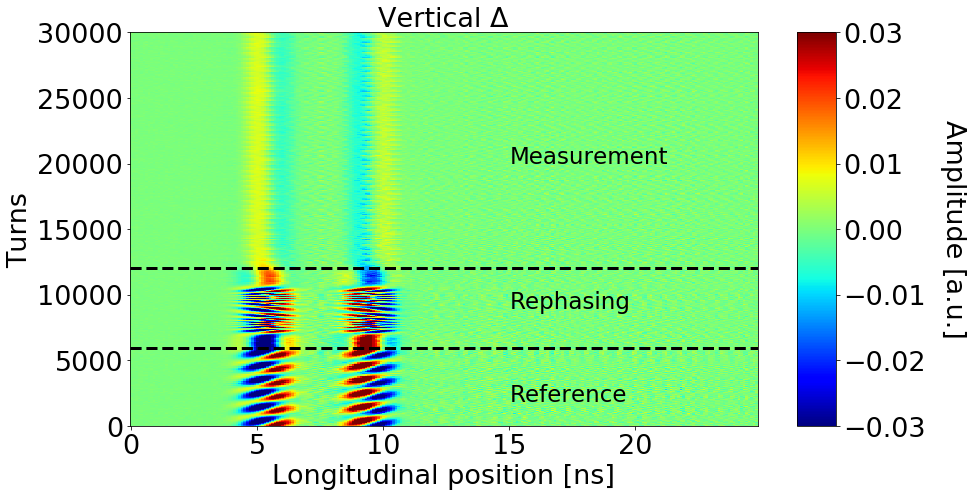
\includegraphics[width=0.8\textwidth]{images/Ch4/HT_measures_vs_reference_vs_corrected__20180530_135105_baseline_correction_onlyDelta.png}
       \caption{HT acquistions before and after the sunchronisation of the SPS main RF with the CC.}
       \label{fig:HT_baseline_correction_measurements_2D}
\end{figure}


\normalsize{\textbf{Headtail monitor callibration}}\\
In order to convert the mean intra-bunch offset ($\Delta$) signal in units of mm the $\Delta$ acquisitions need to be divided by the $\Sigma$ signal and by a normalisation factor which is provided by the callibration of the HT monitor~\cite{PhysRevAccelBeams.22.112803}. The normalisation factor for the SPS was measured at 0.1052 in 2018~\cite{HT_calibration_2018}. Figure~\ref{fig:HT_baseline_correction_crabbing_mm} shows the intra bunch offset from the CC kick in mm and after the baseline correction. Here only the crabbing part is shown and the rest of the signal is discarted.


\begin{figure}[!h]
   \centering         
   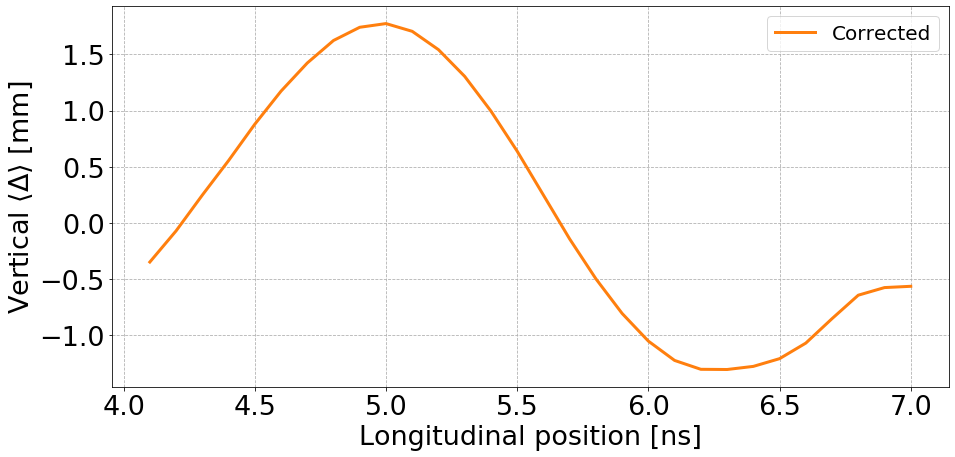
\includegraphics[width=0.8\textwidth]{images/Ch4/HT_measures_vs_reference_vs_corrected__20180530_135105_baseline_correction_mm.png}
       \caption{Intra-bunch offset from the CC kick expressed in mm after the removal of the baseline.}
       \label{fig:HT_baseline_correction_crabbing_mm}
\end{figure}


\normalsize{\textbf{Reconstruction of crabbing}}\\

- Take the measured profile in z
- 
Assuming a trasnverse gaussian distribution and modulating the longitudinal coordinates with the intra-bunch offset measured with the HT monitrore on

- normalised to the maxmimum number of particles over all the longitudinal slices
- x longitudinal slices for 0.1 ns each


 \section{Crab Cavity voltage calibration}\label{sec:Vcc_calibration}

 This section discusses the beam based measurement of the $\CC$ voltage from the HT monitor measurements. The calibration was performed by calculating the kick required to reconstruct the measured intra-bunch offset using Eq.~\eqref{eq:CC_orbit_shift_Chao}. Equation~\eqref{eq:CC_orbit_shift_Chao}, which is obtained from Chaos' Eq... in Ref.~\cite{Chao:1490001}, gives the vertical orbit shift (in meters) from the $\CC$ kick, $\theta$, at the HT monitor location as follows:


\begin{equation}\label{eq:CC_orbit_shift_Chao}
   \Delta y_{,HT} = \frac{\sqrt{\beta_{y, HT}}}{2 \sin(\pi \Qy)} \theta \sqrt{\beta_{y, CC}} \cos(\pi \Qy - \mid \psi_{y, HT} - \psi_{y, CC} \mid),
\end{equation}

where $\beta_y$ is the beta function, $\Qy$ is the tune, and $\psiy$ is the phase advance in tune units. The same applies for the horizontal plane. The indeces HT and CC indicate the optic parameters at the location of the HT monitor and CC respectively.

The deflection from the $\CC$ is written as $\theta = - \frac{q V(t)}{\symE}$, where q is the charge of the particle, $\symE$ the beam energy and $V_{CC}(t) = \VCC \sin(2 \pi \fCC t + \phiCC) $ is the voltage that a particle experiences while passing through the $\CC$. Computing the maximum of $V_{CC}(t)$ gives the cavity voltage, $\VCC$. 

It should be noted here, that the measured intra-bunch offset, $\Delta y_{, HT}$, is inserted in Eq.~\eqref{eq:CC_orbit_shift_Chao} after removing the baseline and converting it in mm as discussed in Section~\ref{sec:HT_info}. Figure~\ref{fig:VCC_from_HT_monitor_measurement} illustrates the cavity voltage computed from the HT signals shown already in this Chapet. Note that the x-axis here doesn't correspond to the 25\,ns slot of the HT acquisition as previously but to the bunch length with $t=0$ at zero crossing. The corresponding beam and optic parameters are listed in Table~\ref{tab:SPS_HT_CC}


\begin{figure}[!h]
   \centering         
   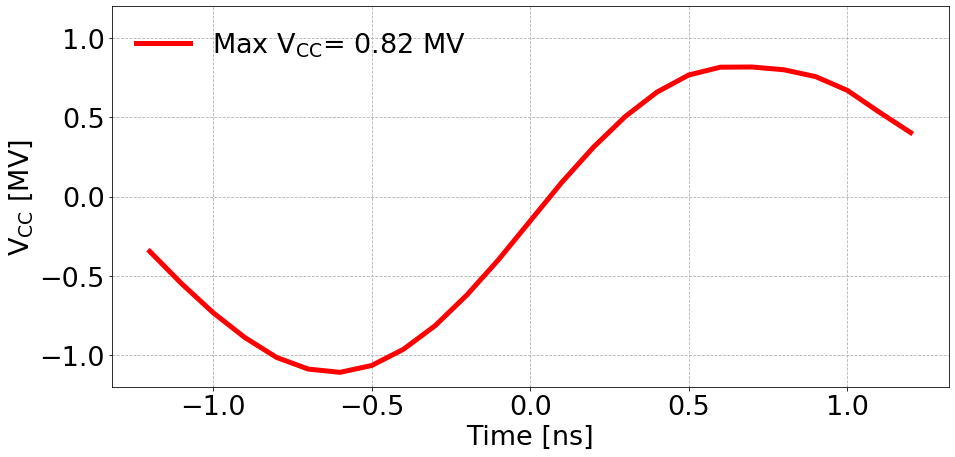
\includegraphics[width=0.8\textwidth]{images/Ch4/HT_VCC__20180530_135105_after_baseline_correction_mm.png}
       \caption{CC voltage measurement from the HT monitor.}
       \label{fig:VCC_from_HT_monitor_measurement}
\end{figure}



\begin{table}[!hbt]
	\centering
   \caption{Parameters for computing the CC voltage from the example HT monitor measurements discussed in this chapter}
	\begin{tabu} to \textwidth { X[c,m] X[c,m] X[c,m] X[c,m] X[c,m] X[c,m] }
		&&&&& \\[-6mm]
		\toprule \toprule
		\multicolumn{2}{l}{\textbf{Parameters}} &
		\multicolumn{2}{c}{\textbf{Units}} &
		\multicolumn{2}{c}{\textbf{Values}} \\
		\bottomrule
      \multicolumn{2}{l}{$\beta_{y, HT}$ / $\beta_{y, CC1}$}& \multicolumn{2}{c}{[m]} & \multicolumn{2}{c}{49.19 / 76.07} \\
      \multicolumn{2}{l}{$\psi_{y, HT}$ / $\psi_{y, CC1}$} & \multicolumn{2}{c}{[-]} & \multicolumn{2}{c}{15.68 / 23.9} \\
      \multicolumn{2}{l}{$\Qy$} & \multicolumn{2}{c}{[-]} & \multicolumn{2}{c}{26.13} \\
      \multicolumn{2}{l}{$\symE$} & \multicolumn{2}{c}{[GeV]} & \multicolumn{2}{c}{26} \\
      \bottomrule
	\end{tabu}
   \label{tab:SPS_HT_CC}
\end{table}



\section{Reconstruction of crabbing}\label{sec:Crabbing_reconstruction}

In this section, the method developed in 2018 to plot a physicall illustration of the crabbing will be described. %This reconstruction of the beam crabbing was a very useful tool for the understadning of the $\CC$ operation and the beam dynamics Ass
Assuming a gaussian transverse profile and modulation the longitudinal coordinates with the intra-bunch offset measured with the HT monitor
%with $\sigma$ computed from the optics at the WS location. 
As discussed in the previous section, the crab cavity voltage can be computed from the HT monitor signal. 

Last, the HT monitor was also used to create a physicall illustration of the crabbing and is shown in this section. 

- Assumes transverse gaussian distribution --> sigma from the emittance the beta gamma and the optics at the location of the WS.


Physicall illustration of crabbing. 
Assuming gaussian transverse distribution. Approximation

Reconstruction of crabbing

\section{Conclusions}


% crab cavity voltage. important for the noise induced emittance growth